\documentclass[border=7pt,varwidth]{standalone}
%\documentclass{article}
\usepackage{tikz}
\usepackage[width=0.5,tiewidth=0.7]{strands}


\newcommand{\fakestar}{*}
\begin{document}

 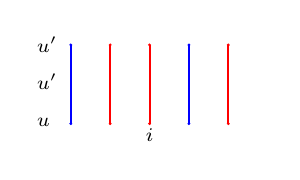
\begin{tikzpicture}[baseline=(current bounding box)]
 \node at (-0.3,0.06) {$\scriptstyle u\phantom{'}$};
 \node at (2.3,0.06) {$\phantom{\scriptstyle u'}$};
 \node at (-0.3,0.53) {$\scriptstyle u'$};
 \node at (-0.3,1) {$\scriptstyle u'$};
 \node at (1,-0.15) {$\scriptstyle i$};
 \node at (1.5,-0.15) {$\phantom{\scriptstyle i+1}$};
 \tie[color=blue,bull=1,bulletie=0.01,style=solid]{{1,1},{1,0}}
 \tie[color=red,bull=1,bulletie=0.01,style=solid]{{2,1},{2,0}}
 \tie[color=red,bull=1,bulletie=0.01,style=solid]{{3,1},{3,0}}
 \tie[color=blue,bull=1,bulletie=0.01,style=solid]{{4,1},{4,0}}
 \tie[color=red,bull=1,bulletie=0.01,style=solid]{{5,1},{5,0}} 
 \end{tikzpicture}
\end{document}